\PassOptionsToPackage{brazil,american}{babel}
\documentclass[12pt]{article}

\usepackage[utf8]{inputenc}

\usepackage{graphicx}
\usepackage{url}
\usepackage{float}
\usepackage{listings}
\usepackage{color}
\usepackage{todonotes}
\usepackage{algorithmic}
\usepackage{algorithm}
\usepackage[hidelinks]{hyperref}

\renewcommand{\contentsname}{Conteúdo}

\title{Proposta de Projeto de Banco de Dados}
\author{Lucas Mafra Chagas}

\begin{document}
	\maketitle
	
	\tableofcontents
	\newpage
	
	\section{Modelo Entidade Relacionamento}
	\subsection{Entidades}
	\subsection{Relacionamentos}
	\subsection{Diagrama Entidade Relacionamento}
	\newpage
	\section{Modelo Relacional}
		\begin{figure}[H]
			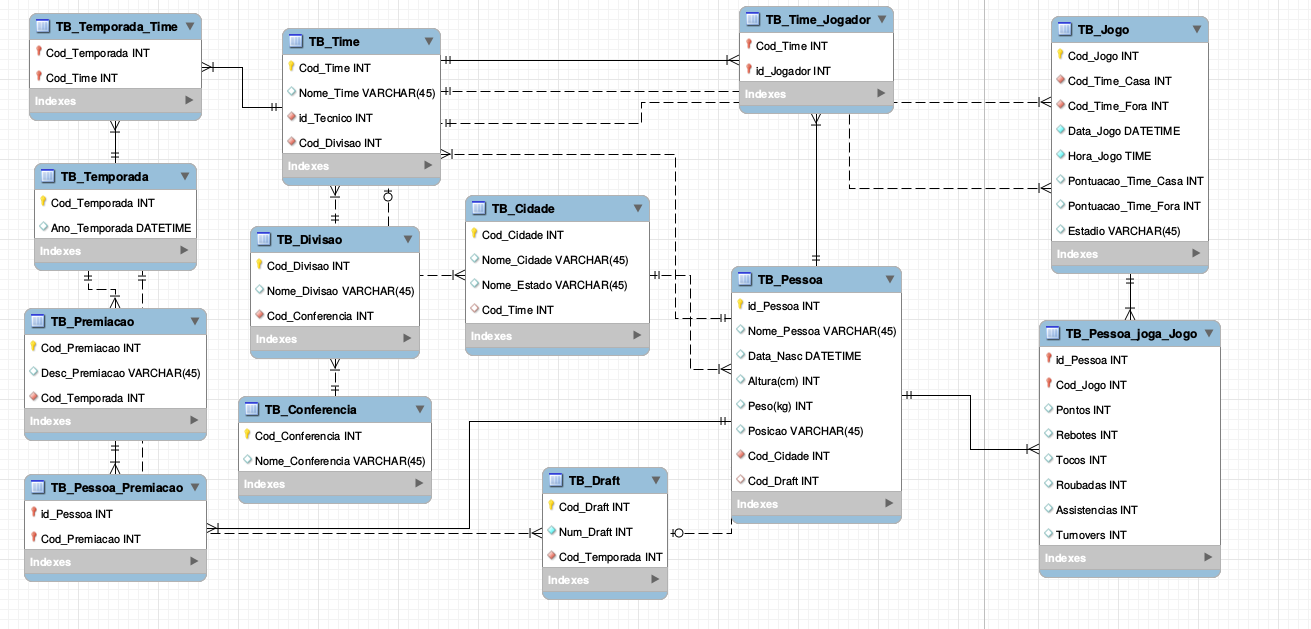
\includegraphics[width=1.0\textwidth]{mrnba.png}
		\end{figure}
	\newpage
	\section{Normalização}
	\newpage
	\section{Álgebra Relacional}
	\newpage
	\section{Referências}
	\begin{itemize}
		\item\textit{\href{http://www.basketball-reference.com/}{Basketball Reference}}: Site com dados referente a Liga Norte Americana de Basquete.
		\item\textit{\href{http://killersports.com/nba/home}{SDQL}}: Banco de Dados criado exclusivamente para esportes americanos.
	\end{itemize}
	\newpage
	
	
\end{document}